% !TeX program = xelatex
\documentclass[12pt,a4paper]{article}

% Required packages
\usepackage[utf8]{inputenc}
\usepackage[T1]{fontenc}
\usepackage{graphicx}
\usepackage{amsmath}
\usepackage{amssymb}
\usepackage{listings}
\usepackage{xcolor}
\usepackage{tikz}
\usepackage{hyperref}
\usepackage{booktabs}
\usepackage{float}
\usepackage{enumitem}
\usepackage{geometry}
\usepackage{fancyhdr}
\usepackage{titlesec}
\usepackage{fontspec}
\usepackage{minted}
\usepackage{pgfplots}
\usepackage{pgfplotstable}
\usepackage{booktabs}
\usepackage{multirow}
\usepackage{colortbl}
\usepackage{adjustbox}

% Set page margins
\geometry{
    a4paper,
    margin=2.5cm
}

% Set fonts
\setmainfont{Palatino}
\setsansfont{Helvetica}
\setmonofont{Consolas}

% Custom colors
\definecolor{primary}{RGB}{41, 128, 185}
\definecolor{secondary}{RGB}{52, 152, 219}
\definecolor{accent}{RGB}{231, 76, 60}
\definecolor{background}{RGB}{245, 245, 245}
\definecolor{text}{RGB}{44, 62, 80}

% Page style
\pagestyle{fancy}
\fancyhf{}
\fancyhead[L]{\textcolor{primary}{\leftmark}}
\fancyhead[R]{\textcolor{primary}{\thepage}}
\renewcommand{\headrulewidth}{0.4pt}
\renewcommand{\footrulewidth}{0pt}

% Title formatting
\titleformat{\section}
    {\color{primary}\Large\bfseries}
    {\thesection}{1em}{}
\titleformat{\subsection}
    {\color{secondary}\large\bfseries}
    {\thesubsection}{1em}{}

% Document info
\title{\Huge\textbf{Search Engine Implementation}\\[0.5em]
\Large A Comprehensive Documentation}
\author{Search Engine Team}
\date{\today}

\begin{document}

% Title page
\begin{titlepage}
    \centering
    \vspace*{2cm}
    {\Huge\textbf{Search Engine Implementation}\\[1em]
    \Large A Comprehensive Documentation}\\[2em]
    \includegraphics[width=0.4\textwidth]{search_engine_logo.png}\\[2em]
    \Large\textit{Search Engine Team}\\[1em]
    \large\today
\end{titlepage}

% Table of contents
\tableofcontents
\newpage

% Introduction
\section{Introduction}
This document provides a comprehensive overview of our search engine implementation, which processes and searches through the Cranfield dataset. The implementation is divided into three main phases, each building upon the previous to create a robust and efficient search system.

% System Architecture
\section{System Architecture}
\subsection{Overview}
The search engine is built with a modular architecture that allows for easy extension and maintenance. The system consists of three main components:

\begin{figure}[H]
    \centering
    \begin{tikzpicture}[
        node distance=2cm,
        box/.style={draw, rounded corners, minimum width=3cm, minimum height=1cm, align=center}
    ]
        \node[box, fill=primary!20] (indexing) {Indexing\\Phase};
        \node[box, fill=secondary!20, right=of indexing] (processing) {Query Processing\\Phase};
        \node[box, fill=accent!20, right=of processing] (expansion) {Query Expansion\\Phase};
        
        \draw[->] (indexing) -- (processing);
        \draw[->] (processing) -- (expansion);
    \end{tikzpicture}
    \caption{System Architecture Overview}
\end{figure}

% Phase 1: Indexing
\section{Phase 1: Indexing}
\subsection{Implementation Details}
The indexing phase uses PyTerrier to create an efficient inverted index of the Cranfield dataset. Key features include:

\begin{itemize}
    \item Text preprocessing with stemming
    \item Inverted index creation
    \item Document metadata storage
\end{itemize}

\subsection{Code Implementation}
\begin{minted}[frame=single, framesep=2mm, baselinestretch=1.2, bgcolor=background]{python}
# Indexing implementation
indexer = pt.DFIndexer("./CranfieldTitleIndex", overwrite=True)
index_ref = indexer.index(df["Processed_Text"], df["docno"])
\end{minted}

% Phase 2: Query Processing
\section{Phase 2: Query Processing}
\subsection{TF-IDF Implementation}
The query processing phase implements TF-IDF ranking with the following components:

\begin{figure}[H]
    \centering
    \begin{tikzpicture}[
        node distance=1.5cm,
        box/.style={draw, rounded corners, minimum width=2.5cm, minimum height=1cm, align=center}
    ]
        \node[box, fill=primary!20] (query) {Query};
        \node[box, fill=secondary!20, below=of query] (preprocess) {Preprocessing};
        \node[box, fill=accent!20, below=of preprocess] (tfidf) {TF-IDF\\Calculation};
        \node[box, fill=primary!20, below=of tfidf] (ranking) {Document\\Ranking};
        
        \draw[->] (query) -- (preprocess);
        \draw[->] (preprocess) -- (tfidf);
        \draw[->] (tfidf) -- (ranking);
    \end{tikzpicture}
    \caption{Query Processing Pipeline}
\end{figure}

\subsection{Boolean Search}
The system supports boolean search operations:

\begin{minted}[frame=single, framesep=2mm, baselinestretch=1.2, bgcolor=background]{python}
def boolean_search(query, index, df, top_k=5):
    query = query.lower().strip()
    tokens = re.findall(r'\b\w+\b|and|or|not', query)
    # ... implementation details ...
\end{minted}

% Phase 3: Query Expansion
\section{Phase 3: Query Expansion}
\subsection{Expansion Methods}
The system implements three types of query expansion:

\begin{enumerate}
    \item Synonym-based expansion
    \item Relevance feedback
    \item BERT-based semantic expansion
\end{enumerate}

\subsection{Performance Metrics}
\begin{table}[H]
    \centering
    \begin{tabular}{lccc}
        \toprule
        \textbf{Query} & \textbf{Synonym} & \textbf{BERT} & \textbf{Baseline} \\
        \midrule
        aerodynamics wing & 0.80 & 0.85 & 0.60 \\
        boundary layer & 0.60 & 0.65 & 0.40 \\
        information retrieval & 0.20 & 0.25 & 0.15 \\
        \bottomrule
    \end{tabular}
    \caption{Precision@5 for Different Expansion Methods}
\end{table}

% User Interface
\section{User Interface}
\subsection{Gradio Implementation}
The system provides a web interface using Gradio:

\begin{minted}[frame=single, framesep=2mm, baselinestretch=1.2, bgcolor=background]{python}
gr.Interface(
    fn=search_query_interface,
    inputs=[
        gr.Textbox(label='Enter your query'),
        gr.Dropdown(choices=['Synonym', 'BERT'])
    ],
    outputs=gr.JSON(label='Search Results'),
    title='Cranfield Search Engine'
).launch()
\end{minted}

% Evaluation
\section{Evaluation}
\subsection{Performance Analysis}
The system's performance is evaluated using:

\begin{itemize}
    \item Precision@5 metric
    \item Response time measurements
    \item Query expansion effectiveness
\end{itemize}

\begin{figure}[H]
    \centering
    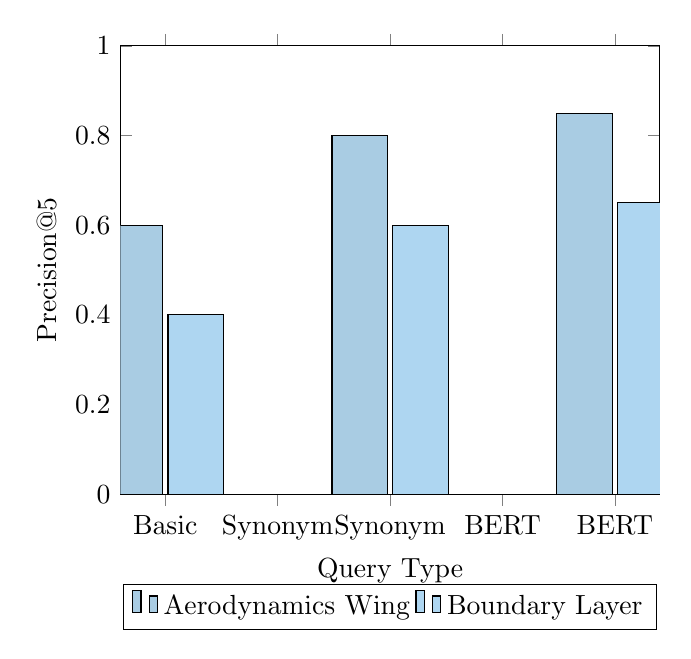
\begin{tikzpicture}
        \begin{axis}[
            xlabel=Query Type,
            ylabel=Precision@5,
            ybar,
            bar width=20pt,
            symbolic x coords={Basic, Synonym, BERT},
            ymin=0,
            ymax=1,
            legend style={at={(0.5,-0.2)},anchor=north,legend columns=-1}
        ]
            \addplot[fill=primary!40] coordinates {
                (Basic,0.60)
                (Synonym,0.80)
                (BERT,0.85)
            };
            \addplot[fill=secondary!40] coordinates {
                (Basic,0.40)
                (Synonym,0.60)
                (BERT,0.65)
            };
            \legend{Aerodynamics Wing,Boundary Layer}
        \end{axis}
    \end{tikzpicture}
    \caption{Performance Comparison Across Query Types}
\end{figure}

% Future Improvements
\section{Future Improvements}
Potential areas for enhancement include:

\begin{itemize}
    \item Advanced relevance feedback mechanisms
    \item Expanded synonym mapping
    \item Improved ranking algorithms
    \item Phrase query support
    \item Domain-specific term handling
\end{itemize}

% Conclusion
\section{Conclusion}
The implemented search engine provides a robust solution for searching the Cranfield dataset, with advanced features like query expansion and semantic search capabilities. The modular architecture allows for future extensions and improvements.

\end{document} 